\documentclass[tikz,border=8pt]{standalone}
\begin{document}
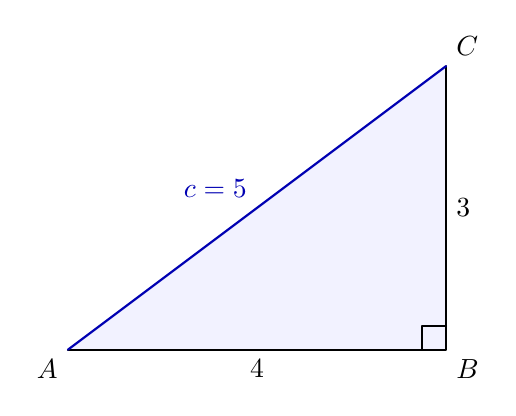
\begin{tikzpicture}[scale=1.2, line cap=round,
  line join=round, thick]
  \coordinate (A) at (0,0);
  \coordinate (B) at (4,0);
  \coordinate (C) at (4,3);
  \fill[blue!5] (A) -- (B) -- (C) -- cycle;
  \draw (A) -- node[below] {$4$} (B)
            -- node[right] {$3$} (C);
  \draw[blue!70!black] (C)
    -- node[above left] {$c=5$} (A);
  \draw (3.75,0) -- (3.75,0.25) -- (4,0.25);
  \node[below left] at (A) {$A$};
  \node[below right] at (B) {$B$};
  \node[above right] at (C) {$C$};
\end{tikzpicture}
\end{document}
